\documentclass[11pt]{article}
\usepackage[a4paper, total={7in, 10in}]{geometry}
\usepackage{amsmath}
\usepackage{graphicx}
\usepackage{hyperref}
\graphicspath{ {./resources/} }
\usepackage[font=small,labelfont=bf]{caption} % Required for specifying captions to tables and figures
\usepackage[T1]{fontenc}
\usepackage[utf8]{inputenc}


\title{Scientific Computing - Finding roots of function}
\author{Mateusz Pełechaty}
\date{23 October 2022}%
\begin{document}
\maketitle


\section{Exercise}
Write a function that finds roots of function by using bisection method
\subsection*{Description}
Bisection is an approximation method that tries to find a root of a function in a given interval. 
It works by repeatedly bisecting the interval in half
and then selecting the subinterval in which the root must lie for further processing.
This method is guaranteed to find a root if the given function is continuous and ends of given interval are 
of different signs. In it's principle it relies on \textbf{Intermediate value theorem (IVT)}
\begin{figure}[h]
    \centering
    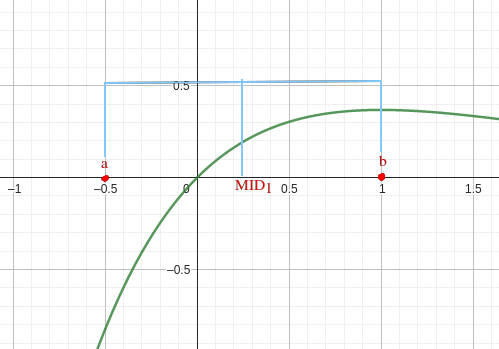
\includegraphics[width=0.5\textwidth]{bisection_example.png}
    \caption{One iteration of bisection method for a = -0.5 and b = 1. The root is in the interval [-0.5, 0.25]}
\end{figure}
\subsection*{Solution and tests}
Function with documentation can be found in \textit{src/roots.jl}\\
Tests can run with \textit{test/test\_roots.jl} and their definitions are in \textit{test/utils.jl}
\section{Exercise}
Write a function that finds roots of function by using newton method
\subsection*{Description}
Newton's method is a technique for finding roots of a functions by upgrading an initial guess to a better approximation of the root.
It is based on the idea that if a function is differentiable, 
then a tangent line to the function at a given point can be used to find a better approximation of the root.
For it to function properly we need to know the derivative of the function and the initial guess which should be close enough to the real root.
\begin{figure}[h]
    \centering
    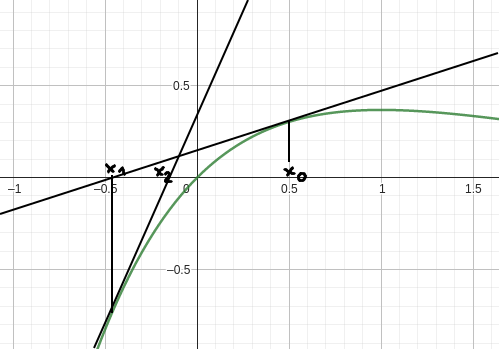
\includegraphics[width=0.5\textwidth]{newton_example.png}
    \caption{One iteration of newton method for a = -0.5 and b = 1. The root is in the interval [-0.5, 0.25]}
\end{figure}
\subsection*{Solution and tests}
Function with documentation can be found in \textit{src/roots.jl}\\
Tests can run with \textit{test/test\_roots.jl} and their definitions are in \textit{test/utils.jl}
\section{Exercise}
Write a function that finds roots of function by using secant method
\subsection*{Description}
The secant method is a root-finding algorithm that uses a succession of roots of secant lines to better approximate a root of a function.
It starts by drawing a secant line between two points, and then uses the intersection of the line and the x-axis as the next approximation.
Two starting approximations should also be chosen close enough to the real root. If they are too far apart, the method may fail to converge.
\begin{figure}[h]
    \centering
    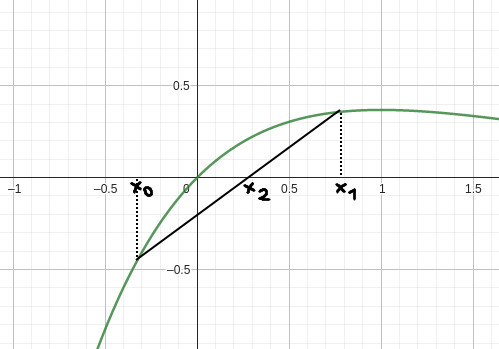
\includegraphics[width=0.5\textwidth]{secant_example.png}
    \caption{One iteration of secant method for a = -0.5 and b = 1. The root is in the interval [-0.5, 0.25]}
\end{figure}
\subsection*{Solution and tests}
Function with documentation can be found in \textit{src/roots.jl}\\
Tests can run with \textit{test/test\_roots.jl} and their definitions are in \textit{test/utils.jl}
\section{Exercise}
Use previously calculated functions to find root of 
$$f(x) = sin x - (\frac{1}{2}x)^2$$
Functions should be called with following arguments:
\begin{itemize}
    \item Bisection method with start range of $[1.5, 2]$ and $\delta = \frac{1}{2}10^{-5}$ and $\epsilon = \frac{1}{2}10^{-5}$
    \item Newton's method with starting approximation of $x_0=1.5$ and $\delta = \frac{1}{2}10^{-5}$ and $\epsilon = \frac{1}{2}10^{-5}$
    \item Secant method with starting approximations of $x_0 = 1$, ${x_1 = 2}$ and $\delta = \frac{1}{2}10^{-5}$ and $\epsilon = \frac{1}{2}10^{-5}$
\end{itemize}
\subsection{Solution and results}
Solution can be found in \textit{src/exercise4.jl}\\
Results can be found in \textbf{Table 1.} and \textbf{Figure 1.}
\begin{table}[!ht]
    \centering
    \begin{tabular}{|l|l|l|l|l|}
    \hline
        \textbf{Method} & \textbf{root} & \textbf{$f(root)$} & \textbf{iterations} & \textbf{error} \\ \hline
        bisection & 1.9337539672851562 & -2.7027680138402843e-7 & 16 & 0 \\ \hline
        newton & 1.933753779789742 & -2.2423316314856834e-8 & 4 & 0 \\ \hline
        secant & 1.933753644474301 & 1.564525129449379e-7 & 4 & 0 \\ \hline
    \end{tabular}
    \caption{Results of finding roots of $f(x) = sin(x) + (\frac{1}{2}\cdot x)^2$}
\end{table}

\begin{figure}[h]
    \centering
    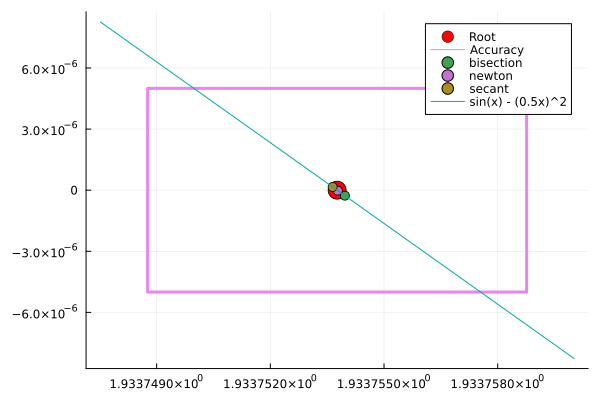
\includegraphics[width=0.5\textwidth]{ex4_plot.png}
    \caption{Results of finding roots of $f(x) = sin(x) + (\frac{1}{2}\cdot x)^2$. Real root was found on WolframAlpha}
\end{figure}
\subsection{Conclusions}
We can see that root finding methods work properly for $f(x) = sin(x) + (\frac{1}{2}\cdot x)^2$.
For test data given as a example, \textbf{newton} method worked best, because it has found asked accuracy with least amount of iterations.

\section{Exercise}
With usage of bisection method, find cross point of functions $f(x) = 3x$, $g(x) = e^x$. Required accuracies: $\delta=10^{-4}$, $\epsilon=10^{-4}$
\subsection{Solution and results}
To compute cross points of $f$ and $g$ we are going to find roots of $f-g$. As there are 2 cross points, we need to find two roots.\\
Solution can be found in \textit{src/exercise5.jl}\\
Results can be found in \textbf{Table 2.} and \textbf{Figure 2.} and \textbf{Figure 3.}\\
\begin{table}[!ht]
    \centering
    \begin{tabular}{|l|l|l|l|l|l|}
    \hline
        \textbf{start\_range} & \textbf{end\_range} & \textbf{found root} & \textbf{f(root)} & \textbf{iterations} & \textbf{error} \\ \hline
        0.0 & 1.0 & 0.619140625 & -9.066320343276146e-5 & 9 & 0 \\ \hline
        1.0 & 2.0 & 1.5120849609375 & -7.618578602741621e-5 & 13 & 0 \\ \hline
    \end{tabular}
    \caption{Roots of $f(x) = e^x - 3x$ calculated by bisection method}
\end{table}
\begin{minipage}{0.8\linewidth}
\begin{minipage}{0.4\linewidth}
    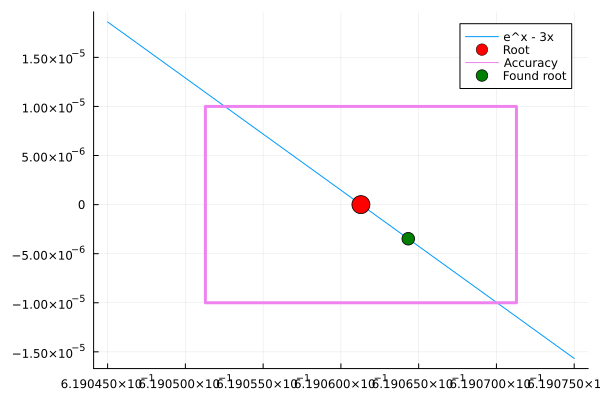
\includegraphics[scale=0.4]{resources/ex5_plot_1}
    \captionof{figure}{Found smaller root}
\end{minipage}
\hfill
\begin{minipage}{0.4\linewidth}
    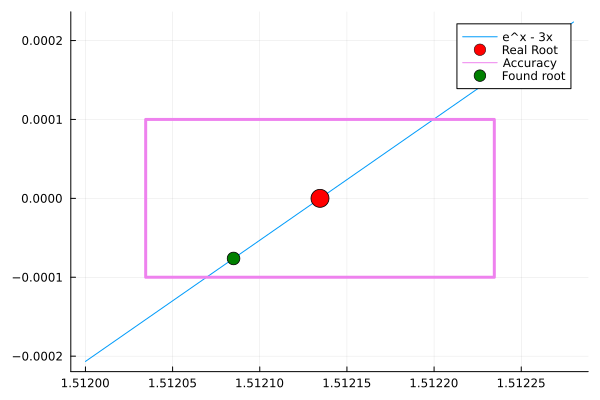
\includegraphics[scale=0.4]{resources/ex5_plot_2}
    \captionof{figure}{Found bigger root}
\end{minipage}
\end{minipage}
\section{Exercise}
\subsection{Task}
Find root of $f_1(x) = e^{1-x} - 1$ and $f_2(x) = xe^{-x}$ by using bisection, Newton and secant methods. Required accuracies: $\delta=10^{-5}$, $\epsilon=10^{-5}$. Choose accordingly starting approximations

\subsubsection{Analysis of functions}
$f_1(x) = e^{1-x} - 1$ has got only one root: $x=1$. For $x>1$ we have $f_1(x) = e^{1-x} - 1 < e^0 - 1 = 0$. For $x < 1$ we have $f_1(x) = e^{1-x} - 1 > e^0 - 1 = 0$. Because of it we are going to use starting approximations that are close to 1.\\
$f_2(x) = xe^{-x}$ has got only one root: $x=0$. For $x > 0$, both $x$ and $e^{-x}$ are positive, so it's product is also positive. For $x < 0$, $f_2(x) < 0$, because product of positive and negative number is negative. Because of it we are going to use starting approximation that are close to 0.\\
\begin{minipage}{1\linewidth}
    \begin{minipage}{0.5\linewidth}
        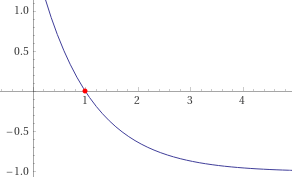
\includegraphics[scale=0.7]{ex6_plot_wolfram_fx}
        \captionof{figure}{$f_1(x)$ drawn on WolframAlpha}
    \end{minipage}
    \hfill
    \begin{minipage}{0.5\linewidth}
        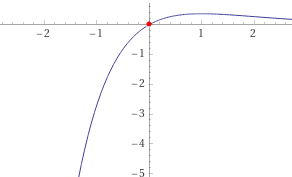
\includegraphics[scale=0.7]{ex6_plot_wolfram_gx}
        \captionof{figure}{$f_2(x)$ drawn on WolframAlpha}
    \end{minipage}
\end{minipage}
\subsubsection{Results of tests}
\begin{table}[!ht]
    \centering
    \begin{tabular}{|l|l|l|l|l|l|l|l|}
    \hline
        function & start\_range & end\_range & delta/epsilon & found root & f(root) & iterations & error \\ \hline
        f & 0.0 & 2.0 & 1.0e-5 & 1.0 & 0.0 & 1 & 0 \\ \hline
        g & -1.0 & 1.0 & 1.0e-5 & 0.0 & 0.0 & 1 & 0 \\ \hline
    \end{tabular}
    \caption{Result of running bisection method on $f$ and $g$}
\end{table}
\begin{table}[!ht]
    \centering
    \begin{tabular}{|l|l|l|l|l|l|l|}
    \hline
        function & $x_0$ & delta/epsilon & found root & f(root) & iterations & error \\ \hline
        f & 0.9 & 1.0e-5 & 0.999999999931772 & 6.822808984452422e-11 & 3 & 0 \\ \hline
        f & 1.1 & 1.0e-5 & 0.99999999991094 & 8.906009263398573e-11 & 3 & 0 \\ \hline
        f & 100.0 & 1.0e-5 & 100.0 & -1.0 & 1 & 2 \\ \hline
        g & 0.5 & 1.0e-5 & -3.0642493416461764e-7 & -3.0642502806087233e-7 & 5 & 0 \\ \hline
        g & 1.1 & 1.0e-5 & 14.272123938290509 & 9.040322779745447e-6 & 3 & 0 \\ \hline
        g & 1.0 & 1.0e-5 & 1.0 & 0.36787944117144233 & 1 & 2 \\ \hline
    \end{tabular}
    \caption{Result of running Newton method on $f$ and $g$}
\end{table}
\begin{table}[!ht]
    \centering
    \begin{tabular}{|l|l|l|l|l|l|l|l|}
    \hline
        function & $x_0$ & $x_1$ & delta/epsilon & found root & f(root) & iterations & error \\ \hline
        f & 0.9 & 1.1 & 1.0e-5 & 1.0000006354049569 & -6.354047550338748e-7 & 3 & 0 \\ \hline
        g & 0.1 & 0.2 & 1.0e-5 & -1.387555849546545e-7 & -1.3875560420776818e-7 & 4 & 0 \\ \hline
    \end{tabular}
    \caption{Result of running Secant method on $f$ and $g$}
\end{table}
\subsubsection{Conclusions}
All methods calculated roots properly if they were set on right starting approximations. Newton method for $x \geq 1$ has not given expected mathematical answer, but it worked as expected. 
\subsection{Question}
What would happen if in Newton method, for $f_1$ we will choose $x_0 \in (1, \infty)$?
\subsubsection*{Answer}
As we can see on \textbf{Table 4.}, if we choose $x_0 = 1.1$ for $f_1$, 
then we get good answer, but on the graph we can see that as $x \rightarrow \infty$ then $f'(x) \rightarrow 0$. 
Because of it, there exists such $x$, that $f'(x) < 1.0e-18$, which is too small for Float64 precision, so $fl(f'(x)) = 0$ and we are going to get an error$=2$ for newton method
\subsection{Question}
What would happen if in Newton method, for $f_2$ we will choose $x_0 > 1$
\subsubsection*{Answer}
If we choose $x_0 > 1$ then Newton's method will try to find root by increasing $x$. It will find one, even though the only root is $x_0 = 1$, because
$g(x)$ gets very close to $0$.  
On \textbf{Table 4.} we can see example when $x_0 = 1.1$. Answer was $root \approx 14.2$ which is nowhere near expected mathematical answer, 
but it has given the right answer, because $f_2(14.2) \approx 0$ for the given delta. Look on the \textbf{Figure 6.} for visualisation for $x_0 = 1.1$ and different accuracies.
Note that for accuracy big enough, $f_2'(x) = 0$ in Float64, so Newton method will give error$=2$ as an output

\begin{figure}[h]
    \centering
    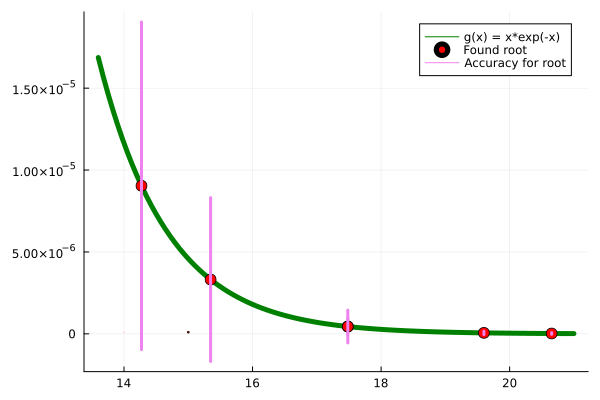
\includegraphics[width=0.5\textwidth]{ex6_3.png}
    \caption{Roots of $f_2(x)$ found by Newton method. $x_0 = 1.1$, accuracies $= \{10^{-5}, \frac{1}{2}10^{-5}, 10^{-6}, \frac{1}{2}10^{-6}, 10^{-7}, \frac{1}{2}10^{-7}\}$}
\end{figure}
\subsection{Question}
Can i choose in Newton method, $x_0 = 1$ for $f_2$ ? 
\subsubsection*{Answer}
If we choose $x_0=1$ for $f_2$ then we are going to get error, because $f_2'(x_0) = 0$. We can also see this on \textbf{Table 4.}
\end{document} 